\documentclass[11pt]{article}
\usepackage{acl2014}
\usepackage{times}
\usepackage{url}
\usepackage{latexsym}
\usepackage{graphicx}
\usepackage{float}
\title{Coconut palms and hand palms: improving similarity ranking by word sense disambiguation}

\author{Anouk Visser \\
  {\tt email} \\\And
  R\'emi de Zoeten \\
  {\tt email} \\}

\date{}

\begin{document}
\maketitle
\begin{abstract}
The abstract will be here.
\end{abstract}

\section{Introduction}

\section{Related Work}
The task of word sense disambiguation is to assign the correct sense to an ambiguous word, whereas word sense discrimination is the task of finding the different senses a word might have \cite{old}. The importance of using co-occurrences for determining the correct sense of a word is already emphasized in \cite{relatedness} in which the authors propose a method for word sense disambiguation using co-occurrences. More specifically, the authors propose a simple score expressing the relatedness between two words:
\begin{equation}\label{r(x,y)}r(x, y) = \frac{f_xy}{f_x+f_y - f_{xy}}\end{equation}
where $f_{xy}$ denotes the frequency of $x$ and $y$ occurring together and $f_x$ and $f_y$ denote the frequency of $x$, respectively $y$. 
In the past years a lot of different methods for word sense disambiguation have been proposed that were either supervised, knowledge-based or unsupervised \cite{survey}. Unsupervised mainly focus on word sense discrimination, the majority of unsupervised word sense discrimination method uses some sort of clustering of for example context vectors or individual words that have a similar meaning. An example of an unsupervised method that uses clustering on both first order context vectors and second order context vectors can be found in \cite{clustering}. Another example of unsupervised word sense discrimination is given in \cite{latent} where the authors use the intuition that the meaning of a word can be represented as a distribution over a set of latent senses.
Recently \cite{word2vec} have released tools for efficiently computing word vectors that capture syntactic and semantic information. The distance between these vectors can be used for identifying linguistic regularities \cite{regularities} and a number of other applications such as word sense discrimination. However, word vector representations suffer from the problem that words may have a number of different meanings that cannot be captured in a single representation. \cite{multi} propose a solution to this problem, they represent a word's meaning by a set of sense specific vectors which are discovered by clustering the contexts in which a word appears. For every context cluster, the authors compute an average vector that can be used to determine the similarity between two words (either in context or isolated). The size of the set of sense specific vectors is set in advance and is the same for every word. \cite{global} build upon this work by introducing a new neural network architecture that learns word vectors that also incorporate the global context of a word and can lean multiple vectors for a single word. In addition to this, they present a new dataset of pairs of words in contexts annotated with similarity judgements by human annotators. 

\section{Training data}
For model training data we used the enwiki8 dataset \cite{enwiki} corpus. For our purposes we filtered the corpus to only keep the words in the following Part-Of-Speech categories: Nouns, Verbs, Adjectives and Adverbs. We think that these words are more relevant for the task of word sense disambiguation and that words from other categories (such as the determiners) would only add noise to our models. Furthermore, we lemmatized all words so that e.g. \textit{computer}, \textit{computers} and \textit{computing} are all projected onto the token \textit{comput}. The lemmatization is used as a form of dimensionality reduction.

\section{COCONUT}
%COPIED FROM REPORT ULL (SHOULD BE ADJUSTED)
The COCONUT method for disambiguating words is based on two assumptions: 
\begin{enumerate}
\item the meaning of a word is highly dependent on the words it co-occurs with
\item the co-occurring words that define one meaning of a word are more likely to co-occur with each other than two words that define two different meanings of the word
\end{enumerate}

Let $C$ be the set of words that co-occur with $A$, the word we want to disambiguate. COCONUT first constructs and converts the global co-occurrence vectors of the words in $C$ to relatedness vectors. It will then cluster these relatedness vectors in order to determine the two possibly different meanings of $A$. 

\subsection{Co-Occurrence Vectors}
A global co-occurrence vector contains the frequencies indicating how many times two words co-occur, we convert the absolute frequencies in the global co-occurrence vector to a relatedness score. We use the same function for relatedness as \cite{relatedness}.

Words that are not closely related to $A$ do not contribute to either one of the meanings. Therefore, we will discard the words that have a relatedness score with $A$ that falls in the bottom $50\%$ of all relatedness-scores from $C$. The terms that are discarded are considered relevant to all meanings of $A$, we will call this set $R$.

\subsection{Clustering and splitting}
Let the set of co-occurrence vectors from the words in $C$, be called $V$. After applying k-means clustering on the vectors in $V$ we expect to find two cluster centers that represent the two meanings for $A$. Note that we are only interested in describing the two meanings of $A$ using the words in $C$. Therefore, for every vector in $V$ we will discard all words that are not in $C$. The adjusted vectors can now be used to perform k-means clustering. 

The two new co-occurrence vectors for $A$ are initialized with the words in $R$. As the cluster centers define the different meanings of $A$, we can look at the words in each cluster to fill the new co-occurrence vectors for $A$.  

COCONUT will split every word in the corpus in order to find two different meanings (we excluded the 75 most frequent words), but not all words are ambiguous. We expect that words that have two distinct meanings will have a greater cluster distance (i.e. a greater distance between the two meanings) than words that do not. We discard all disambiguations for the words that have a cluster distance that falls in the bottom $50\%$ of all cluster distances.
\begin{figure*}
\center
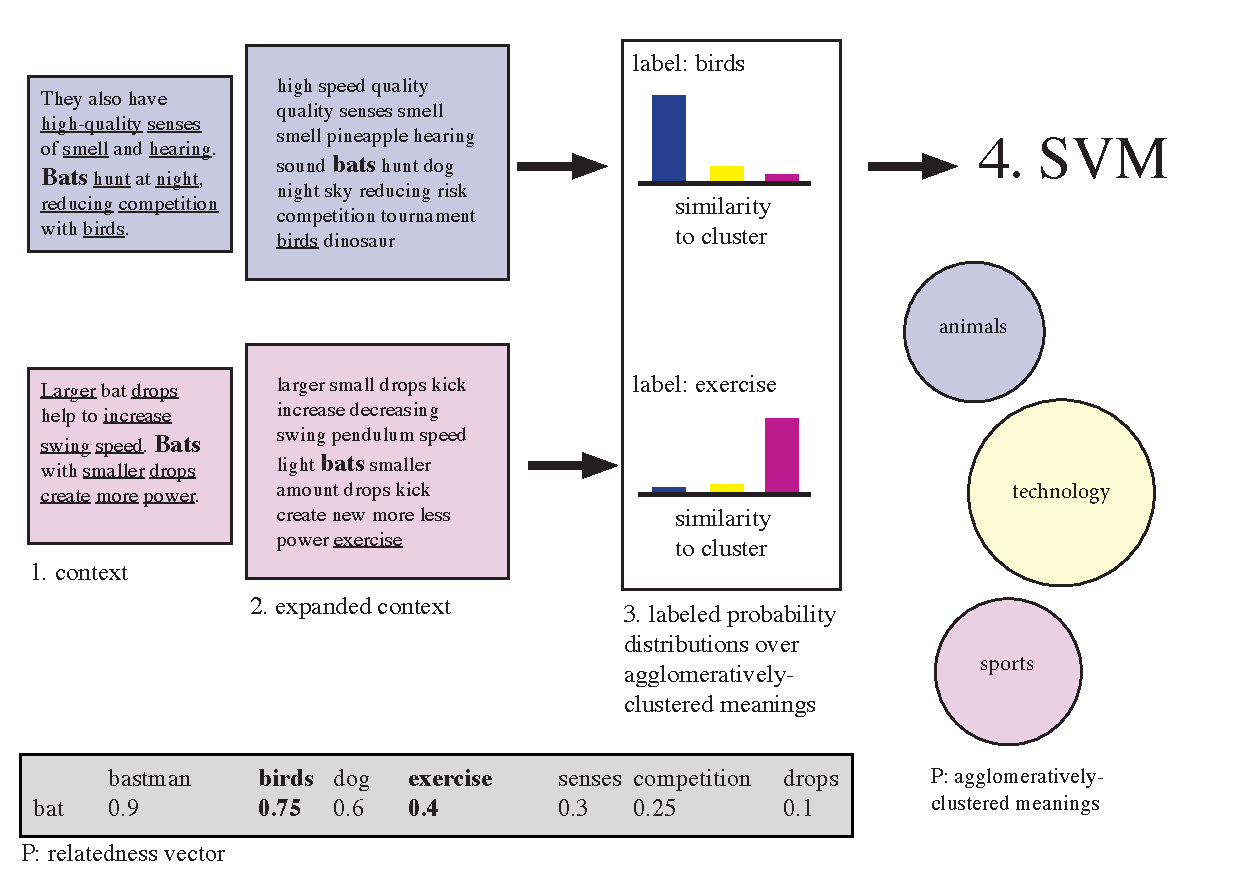
\includegraphics[scale=0.75]{images/palm.pdf}
\caption{The five steps of the PALM algorithm. P: preprocessing, PALM requires agglomeratively-clusterd latent meanings and relatedness vectors for all words in the corpus. 1. Extract every context word $W$ appears in. 2. Expand the context. 3. Choose a label from the expanded context and create a `histogram' over the agglomeratively-clusterd latent meanings for every expanded corpus. 4. Train an SVM on these histograms using the labels.}
\label{palmimg}
\end{figure*}

\section{Agglomerative Clustering}
One way to cluster data is agglomerative clustering which has been shown to produce good results in comparison with other clustering techniques \cite{clustering}. Agglomerative clustering is an iterative bottom up approach to clustering. At the start each data point forms its own cluster and in each iteration the two data points that are closest to each other are merged until there is only a given number of clusters or the inter-cluster distances are larger than a predefined value. We performed agglomerative clustering on the $80$ dimensional word vector representations that we extracted from our training data. We clustered the words into 500 clusters. The result was that 351 clusters were single word clusters. The distribution over the number of words in each cluster is skewed and clusters with one or just a few words in them are not informative. Therefore we removed the clusters that had less than $10$ words in them, which resulted in 41 clusters with a distribution over the cluster size shown in figure \ref{cluster_size}.
\begin{figure}[H]
\center
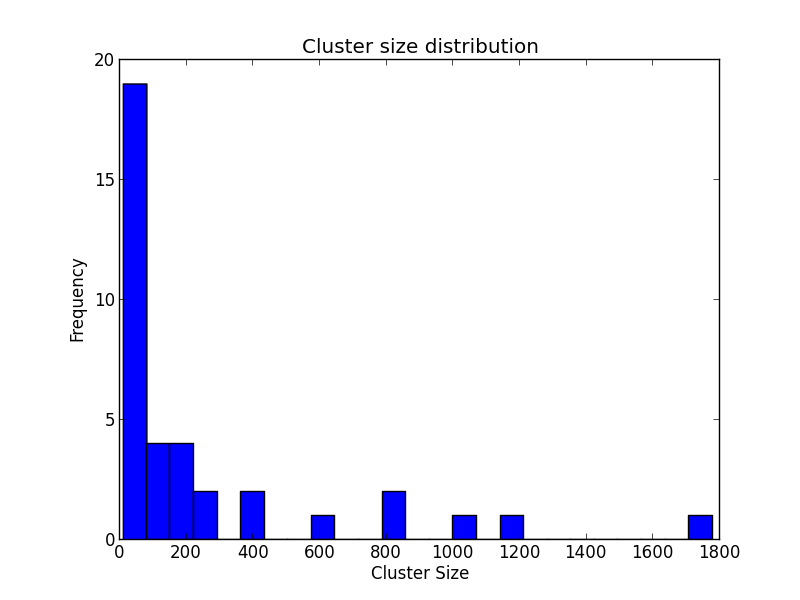
\includegraphics[scale=0.40]{images/cluster_size.png}
\caption{Distribution over cluster sizes for agglomerative clustering.}
\label{cluster_size}
\end{figure}
For each of the tasks we compare the context of the word that needs to be disambiguated with all the clusters. We determine the likelihood of a context $cont$ being represented by a cluster by counting how many words are in common with the cluster:

\begin{equation} \label{pcc}P( cluster | cont ) = \frac{ | \{cluster \cap cont\} |  }{| cluster |} \end{equation}

By applying \ref{pcc} to all clusters for a given context and normalizing over the different probabilities we get a probability vector $V_{c}$ that defines a mixture of the context over the different clusters. It is then possible to define a similarity between the two contexts $V_{c_1}$ and $V_{c_2}$ by their cosine similarity $cos(V_{c_1}, V_{c_2})$.

\section{PALM}
In order to disambiguate between multiple meanings of a word, it can be useful to look at the context. PALM is a method for word sense discrimination that trains an SVM for every word that given a context predicts a label that describes the meaning of the word. These labels can be used to relabel a corpus before training a recurrent neural network to obtain multiple vector representations for one word. In this section we describe the PALM method in detail, figure \ref{palmimg} provides an overview of the algorithm. 

\subsection{Choosing the label}
Let $W$ be the word for which we want to train the SVM. PALM starts by extracting all contexts that $W$ appears in. We define `context' as all words within a window around $W$ (in our experiments we looked five words back and five words ahead). Our aim is to assign a label to each of these contexts that describes the sense of the words best, the collection of labels then represent the different sense a word can have. As we have seen in \cite{analysis} underspecified contexts are often observed. In line with our assumption for the COCONUT baseline (i.e. the co-occurring words that define one meaning of a word are more likely to co-occur with each other than two words that define two different meanings of the word) we expand the context by adding the $n$ (in our experiments we set $n=5$) most related words to every word in the context (except for $W$). Finally, a word from the expanded context is selected as a label so that:
$$label = \arg\max_w \frac{r(W, w) + \textit{sim}(W, w)}{2}$$
where $\textit{sim}(W, w)$ denotes the cosine similarity between $W$ and $w$. 

\subsection{Probability distribution over agglomeratively-clustered latent meanings}
% Change this part a bit so that it is not like we have a large number of vectors to start with. Actual implementation can be different from description.
For every word in the expanded context we find the similarity to every agglomeratively-clustered latent meaning, creating an $N$ dimensional vector (where $N$ is the number of agglomeratively-clustered latent meanings that were found). These vectors are accumulated and normalized, so that we have one vector for every context. 
\begin{equation}\label{pa}m_i = \frac{1}{N_c}\sum\limits_{w\in C}sim(w, m_i)\end{equation}
Although the values denote the accumulated similarity of the words from the expanded context to the meanings, we can interpret the vector as a probability distribution over meanings, given the context (when the context and a meaning are very similar, it is very likely that the context imposes this meaning). 

\subsection{Label reduction}
The last step before training the SVM consists of reducing the number of labels. Although including the second-order context by expanding the context radically decreases the number of new labels, there will still be many labels including a number of labels that describe the same sense of $W$. We have implemented a method for label reduction that favors labels that were observed most frequently. We iteratively split the labels into two halves: the upper half (containing labels that were seen most frequently) and the lower half (containing labels that were seen least frequently) and merge a label (and all of its vectors) from the lower half ($w_l$) into a label form the upper half ($w_u$). $w_l$ and $w_u$ are chosen by: 
$$\arg\max_{w_l, w_u} \textit{sim}(w_l, w_u)$$
This process continues until $\textit{sim}(w_l, w_u)$ is below a certain threshold (in our experiments the threshold was $0.5$).
The reordered labelled data can then be used to train an SVM. The SVM can then disambiguate a word by predicting a the most appropriate label given the probability distribution from an expanded context over the agglomeratively-clustered latent meanings. 
%\section{REMI}

\section{Experiments}

\section{Quantitative evaluation}
We evaluate the performance of our WSD methods on the dataset constructed by \cite{global}. The dataset consist of 2003 word pairs and their context. The goal of the task is to assign a similarity measure to all word pairs. 241 word pairs consist of the same word, there are a total of 1712 unique words. Ten human judges assigned similarity scores to all word pairs. We compute the Spearman correlation between the method's similarity ratings and the average of the human annotators. We compare our methods to a baseline that uses only a single word vector for every word and computes the similarity as the cosine similarity between the two words without taking the context into account. 

To compute the score for PALM we applied the word sense discrimination on the X corpus. PALM was able to identify different senses for 1222 of the 1712 unique words of the word pairs, resulting in 1222 SVMs. We then relabeled the 1222 words in the X corpus by appending the label predicted by the SVM for the word after extracting its probability distribution over meanings. Finally, we used \textit{word2vec} by \cite{word2vec} to obtain 80-dimensional word vectors for all words in the relabeled corpus. To compute the similarity of the word pair, we expand the contexts of both words use this to compute the probability distribution over the meaning. The trained SVM then provides the label of the word vector that represents the words best in their given contexts. 

\section{Discussion and future work}
\section{Conclusion}

\bibliographystyle{acl}
\bibliography{cocobib}

\end{document}
